\documentclass{standalone}
\usepackage{pgfplots}
\usepgfplotslibrary{groupplots,fillbetween}
\usepackage{animate}

\usepackage{pgf}
\usepackage{tikz}

\usetikzlibrary{fit}
\usetikzlibrary{positioning}
\usetikzlibrary{arrows}
\usetikzlibrary{automata}
\usetikzlibrary{backgrounds}
\usetikzlibrary{shapes.misc}

\begin{document}

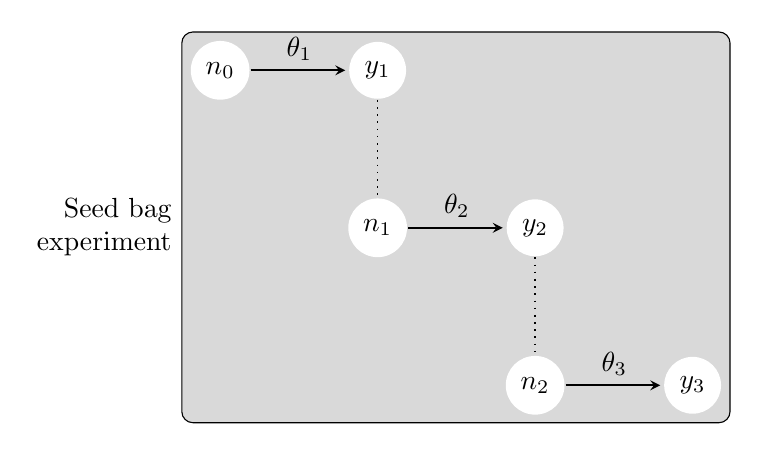
\begin{tikzpicture}[
            > = stealth, % arrow head style
            shorten > = 1pt, % don't touch arrow head to node
            auto,
            node distance = 2cm, % distance between nodes
            semithick % line style
        ]

        \tikzstyle{every state}=[
            draw = none,
            thick,
            fill = white,
            minimum size = 4mm
        ]

	% START OF SEED BAG EXPERIMENT
        \node[state] (N0) [] {$n_0$};

	% AGE 1 SEED BAG ESTIMATES      
        \node[state] (Y1) [right of=N0] {$y_1$};
        \node[state] (N1) [below of=Y1] {$n_1$};
        \node[state] (Y2) [right of=N1] {$y_2$};
        \node[state] (N2) [below of=Y2] {$n_2$};
        \node[state] (Y3) [right of=N2] {$y_3$};
        
        \path[->] (N0) edge node {$\theta_1$} (Y1);
        \path[->] (N1) edge node {$\theta_2$} (Y2);
        \path[->] (N2) edge node {$\theta_3$} (Y3);

        \path[dotted,-] (Y1) edge (N1);
        \path[dotted,-] (Y2) edge (N2);

       	\begin{scope}[on background layer]
	\node[draw,fit=(N0) (Y3) , fill = gray!30, rounded corners, inner sep = .1cm, label={[label distance=0cm, align = right]left:{Seed bag \\ experiment}}] {};
	  \end{scope}

  \end{tikzpicture}
    
  \end{document}